\documentclass[a4paper, 10pt]{article}
\usepackage[utf8]{inputenc}
\usepackage[T1]{fontenc}
\usepackage[french]{babel}
\usepackage{graphicx}
\graphicspath{ {images/} }
\usepackage{amssymb, bm}
\usepackage{subcaption}
\usepackage{caption}
\usepackage{float}


\title{CSOPT : Calcul scientifique et optimisation \\ Travaux pratiques \\ Optimisation sans contraintes }
 \author{Yassine Jamoud \and Samy Haffoudhi}

\begin{document}

	\maketitle
	
	\newpage
	
	\section{Minimisation de la fonction de Rosenbrock}
			$$
			f_0(x)= \sum_{i=1}^{n-1} b(x_{i+1}-x_i^2)^2 + (1-x_i)^2, \;\;\;\;    \forall x \in \mathbb{R}^n \mbox{ et b }  \in \mathbb{R}^+.
			$$
		\subsection{Travail préliminaire}
			\begin{enumerate}
				\item{
					De manière générale 
					$$
					\nabla f(x) = \left[
					\begin{array}{c}
					-4bx_1(x_2-x_1^2)-2(1-x_1) \\
					2b(x_2-x_1^2)-4bx_2(x_3-x_2)-2(1-x_2) \\
					\vdots \\
					2b(x_n-x_{n-1}^2)-4bx_n(x_{n+1}-x_n^2)-2(1-x_n)
					\end{array}
					\right]
					\;\;\;\;\;
					\nabla ^2 f(x)=
					$$
					Soit pour n = \textbf{2}, $ \;\;\;\;  f_0(x) = b(x_2-x_1^2)^2+(1-x_1)^2, \;\;\;\;    \forall x \in \mathbb{R}^2 \mbox{ et b }  \in \mathbb{R}^+.$
					$$
					\nabla f(x) = \left[
					\begin{array}{c}
					-4bx_1(x_2-x_1^2) - 2(1-x_1)\\
					2b(x_2-x_1^2)
					\end{array}
					\right]
					\;
					\nabla ^2f(x)=\left[
					\begin{array}{cc}
					-4b(x_2-x_1^2)+8bx_1^2 +2 & -4bx_1\\
					-4bx_1 & 2b
					\end{array}
					\right]
					$$
				}
				
				\item{
					Pour trouver le minimiseur, on cherche à annuler le gradient :
					$$
						\nabla f_0(x_0)=0 \;\;\; \Rightarrow  \;\;\;
						\left\{
							\begin{array}{rl}
								-4bx_1(x_2-x_1^2)-2(1-x_1)= 0 \\
								2b(x_2-x_1^2) =0
							\end{array}
						\right. \;\;\; \Rightarrow \;\;\; \left\{
							\begin{array}{rl}
								x_2 = x_1^2 \\
								1-x_1 =0
							\end{array}
							\right.
					$$
					D'où $x_0= \left[ \begin{array}{c} 1 \\ 1  \end{array} \right]$ avec $f_0(x_0) = 0$
				}
				\item{
					On pose $f_0$ sous la forme d'un critère de moindres carrés non-linéaires tel que $f_0(x)=\frac{1}{2}r_1^2(x) + \frac{1}{2}r_2^2(x)$
					\\ \\
					On a alors $r(x) = \left[ \begin{array}{c} \sqrt{2b}(x_2-x_1^2) \\ \sqrt{2}(1-x_1) \end{array} \right]$
					\\Le Jacobien s'exprime comme $J=\left[ \begin{array}{cc} \frac{ \partial r_1}{\partial x_1} &  \frac{ \partial r_1}{\partial x_2} \\ \\ \frac{ \partial r_2}{\partial x_1} & \frac{ \partial r_2}{\partial x_2} \end{array} \right]$
					\\ \\ Après calcul on obtient alors :
					$$
					J=\left[
					\begin{array}{cc}
						-2x_1\sqrt{2b} & \sqrt{2b} 
						\\ \\
						-\sqrt{2} & 0 \frac{ \partial r_1}{\partial x_2} 
					\end{array} \right]
					$$
					
				}
			\end{enumerate}
		\subsection{Visualisation de la fonction objectif}
			On trouve alors pour $x_1 \in \left[ -4, 4 \right] \mbox{ et } x_2 \in \left[ -5, 20 \right]$
			\newline
			\begin{figure}[h]
				\centering
				\begin{subfigure}[h]{0.49\textwidth}
         				\centering
         				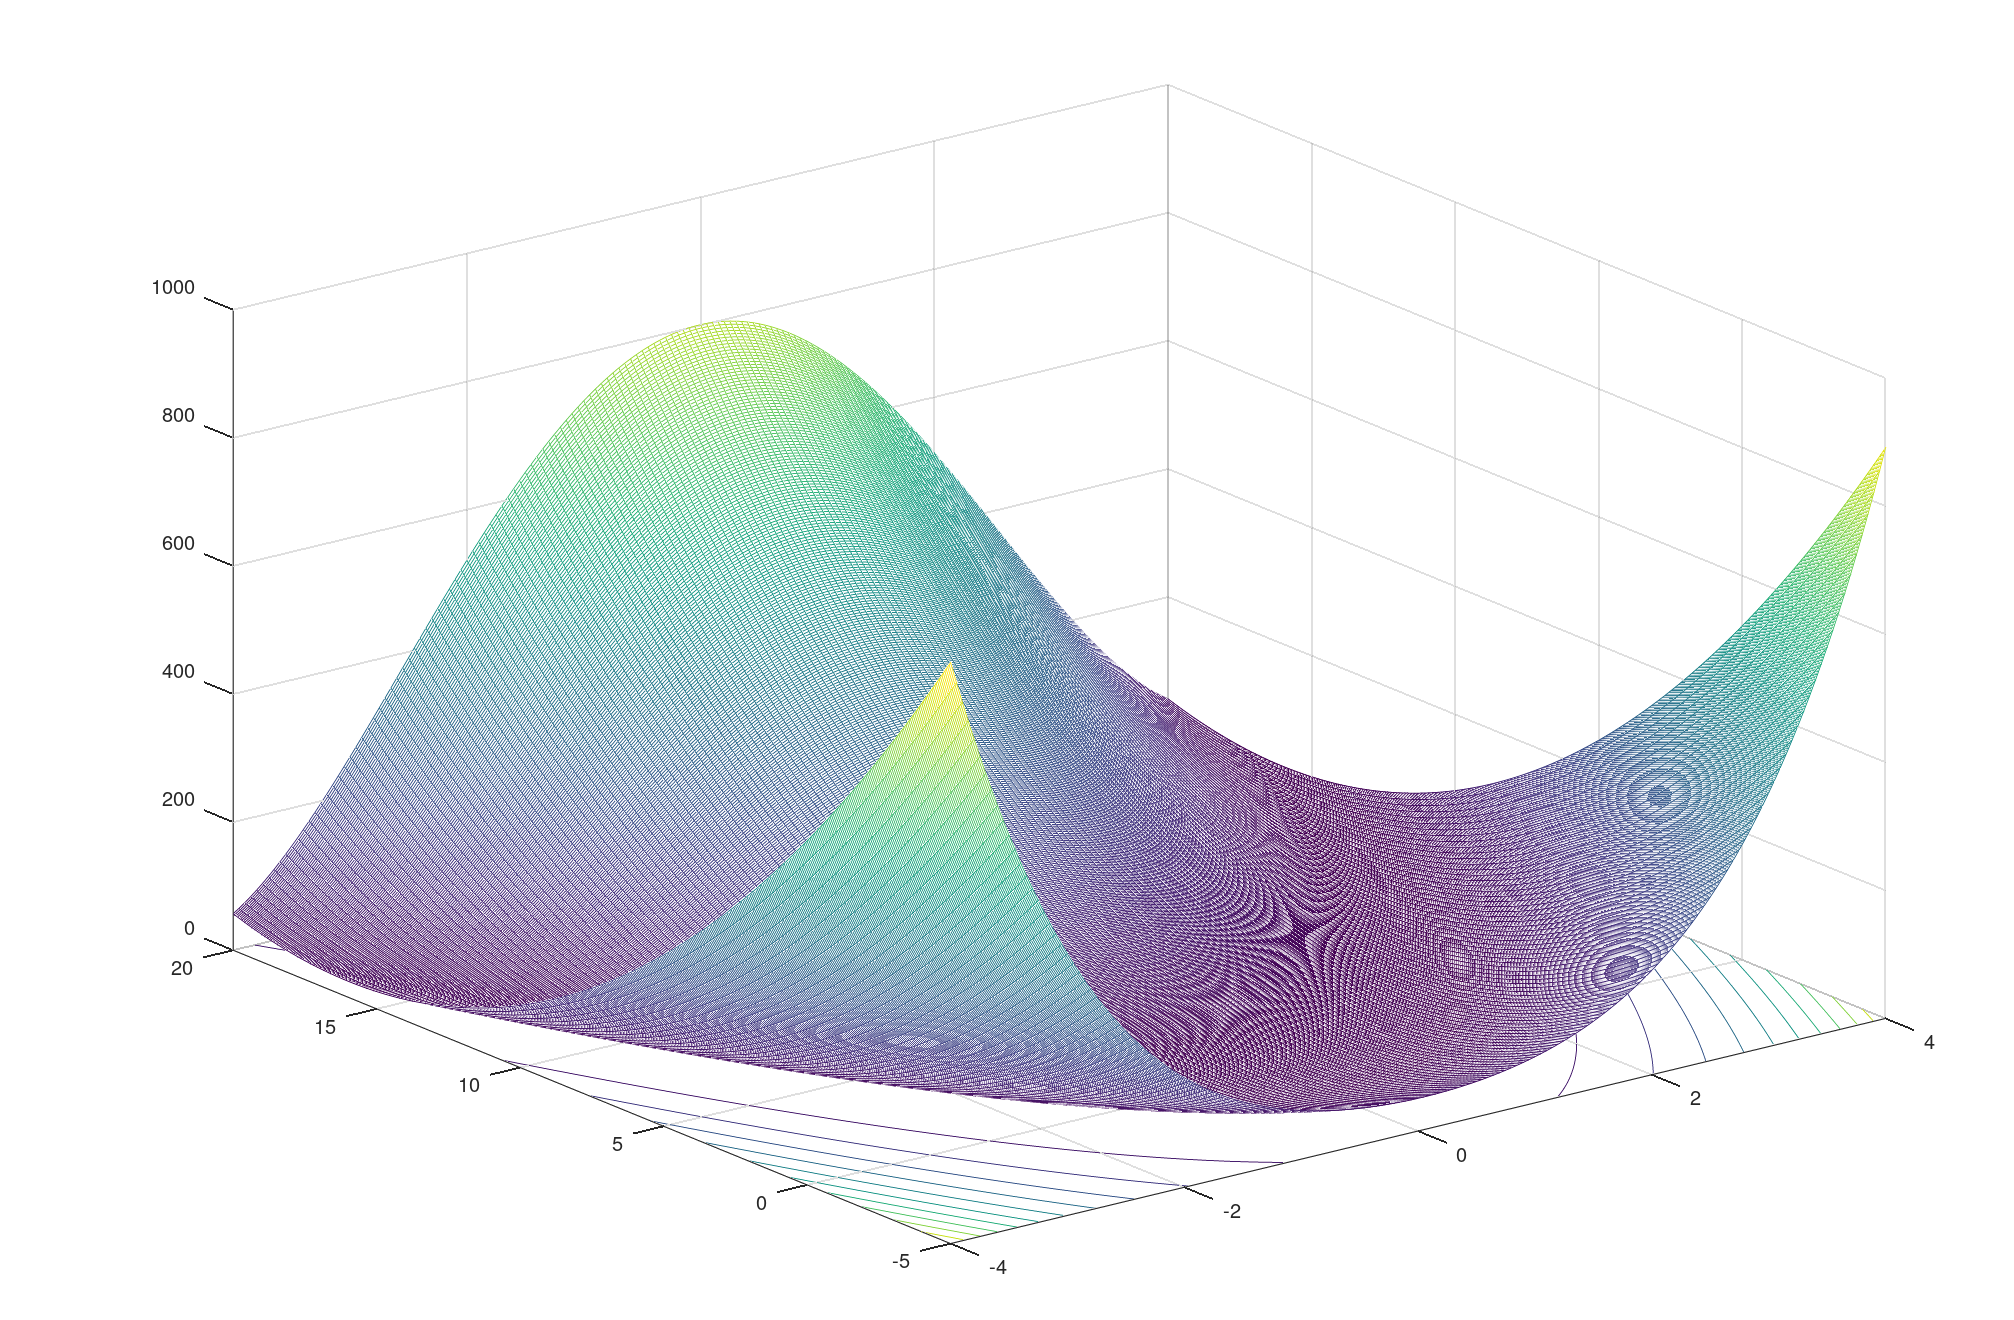
\includegraphics[width=\textwidth]{rosenbrock3D}
         				\caption{Visualisation de la fonction de Rosenbrock en 3D}
     				\end{subfigure}
				\begin{subfigure}[h]{0.49\textwidth}
         				\centering
         				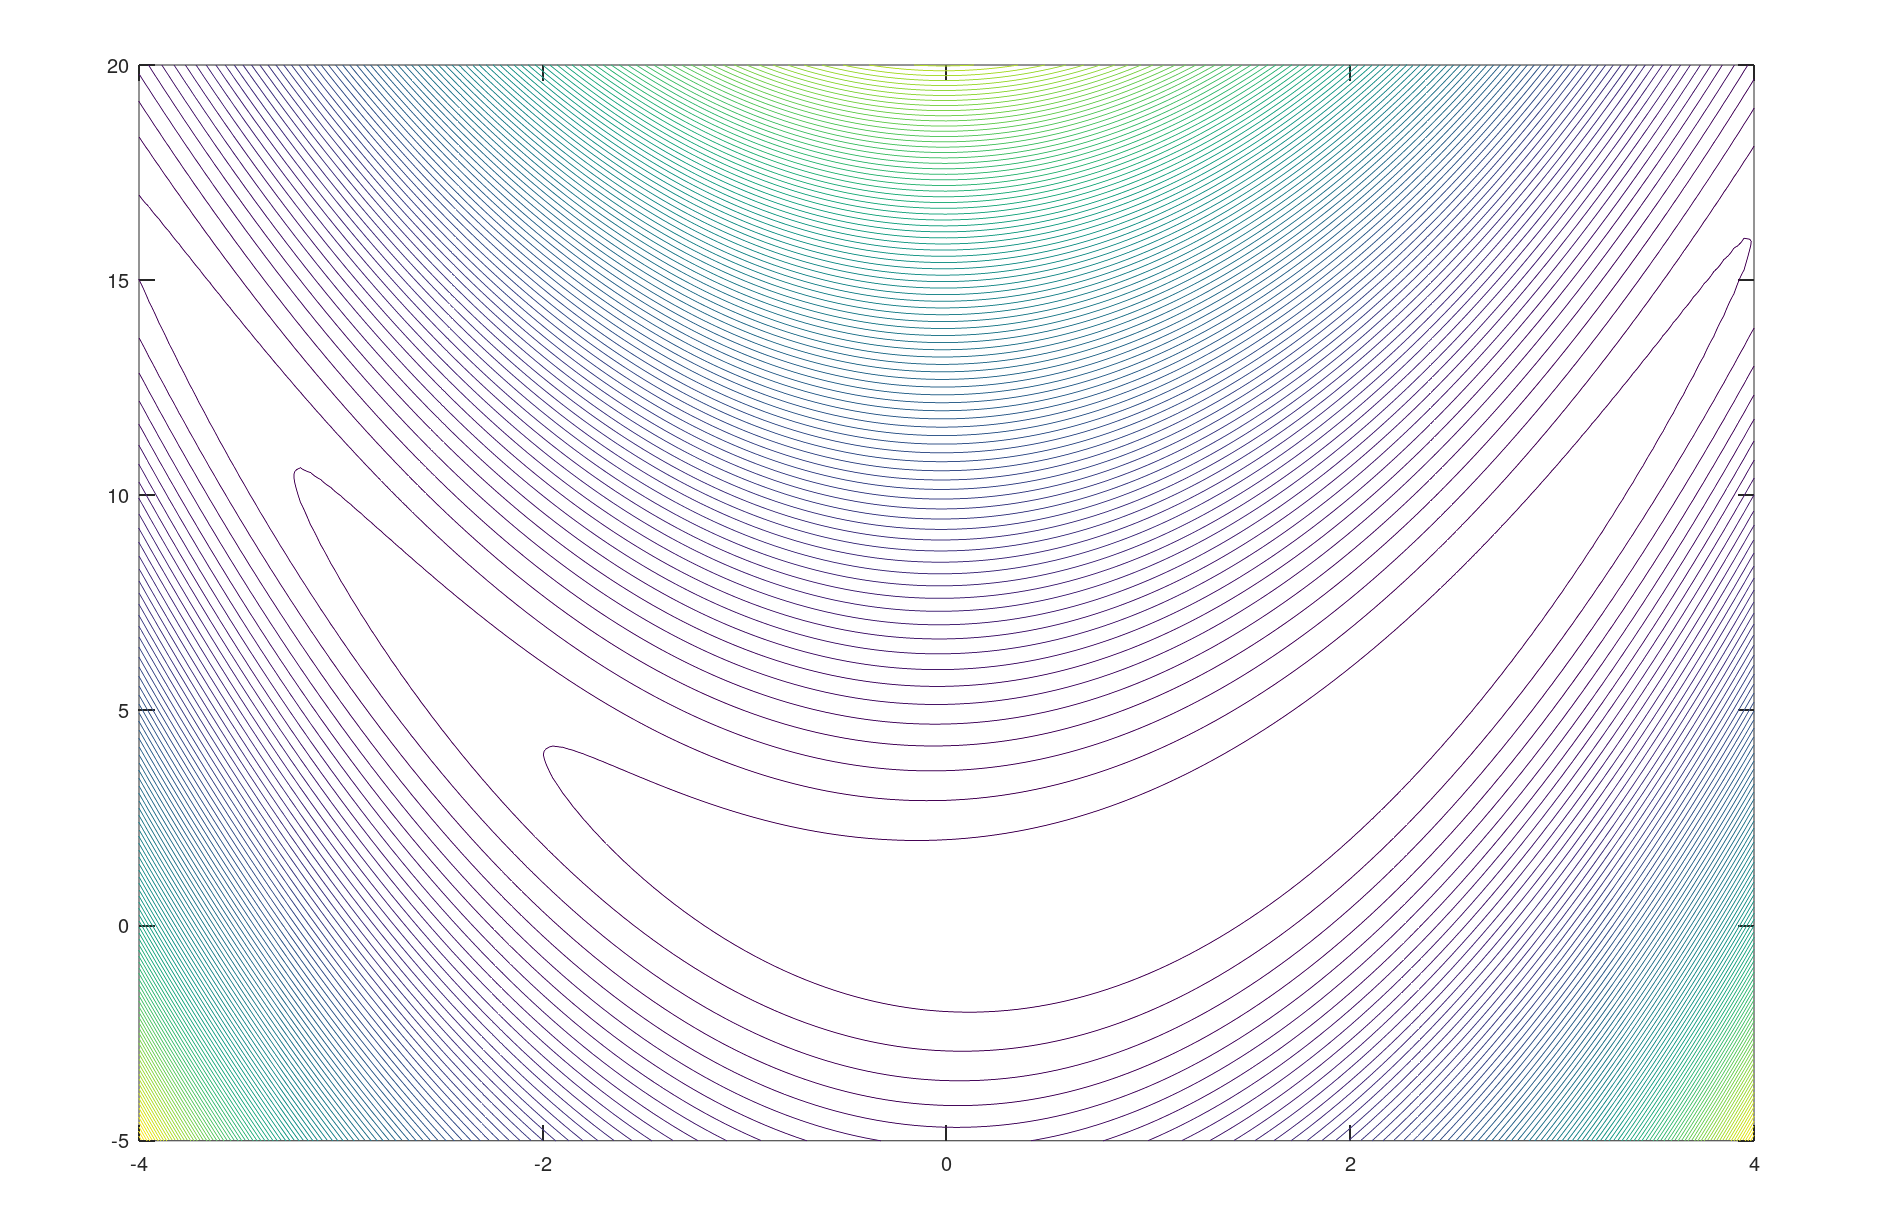
\includegraphics[width=\textwidth]{contourRosenbrock}
         				\caption{Visualisation des lignes de niveaux de la fonction}
     				\end{subfigure}
			\end{figure}
			
		\subsection{Minimisation par descente itérative}
		Pour commencer, on utilise la méthode de descente de plus forte pente avec un pas fixe.
		On obtient alors en 1000 itérations les différents figures : 
		\begin{figure}[H]
			\centering
			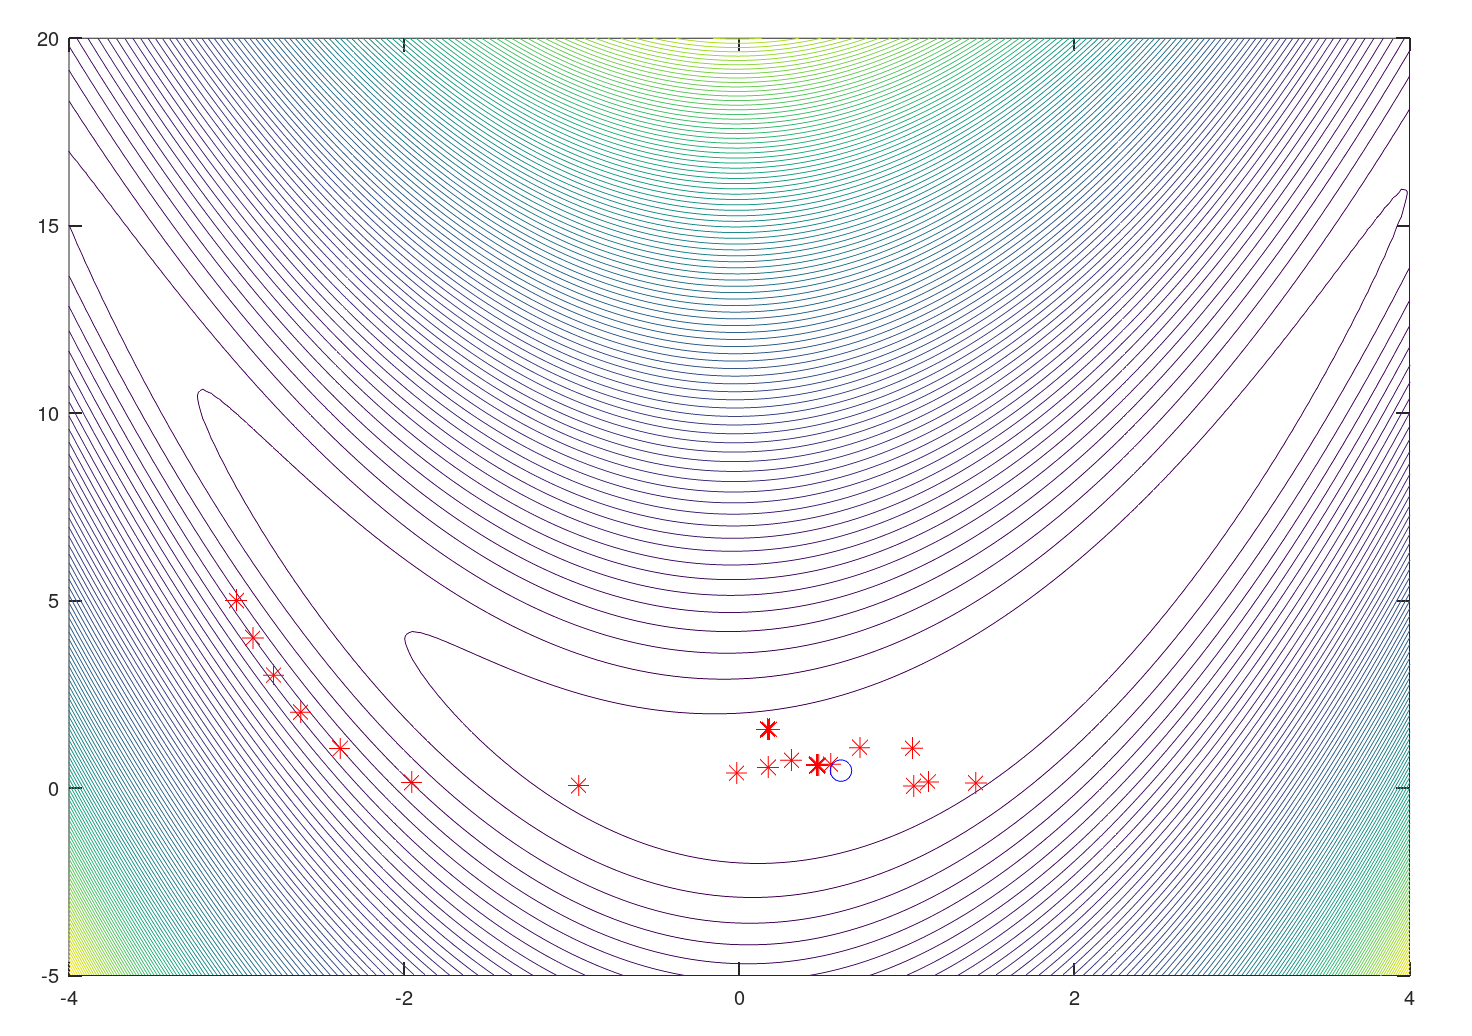
\includegraphics[width=7cm, height=4cm]{pasFixe1}
			\caption{Descente de pas 1}
		\end{figure}
		
		\begin{figure}[H]
			\centering
			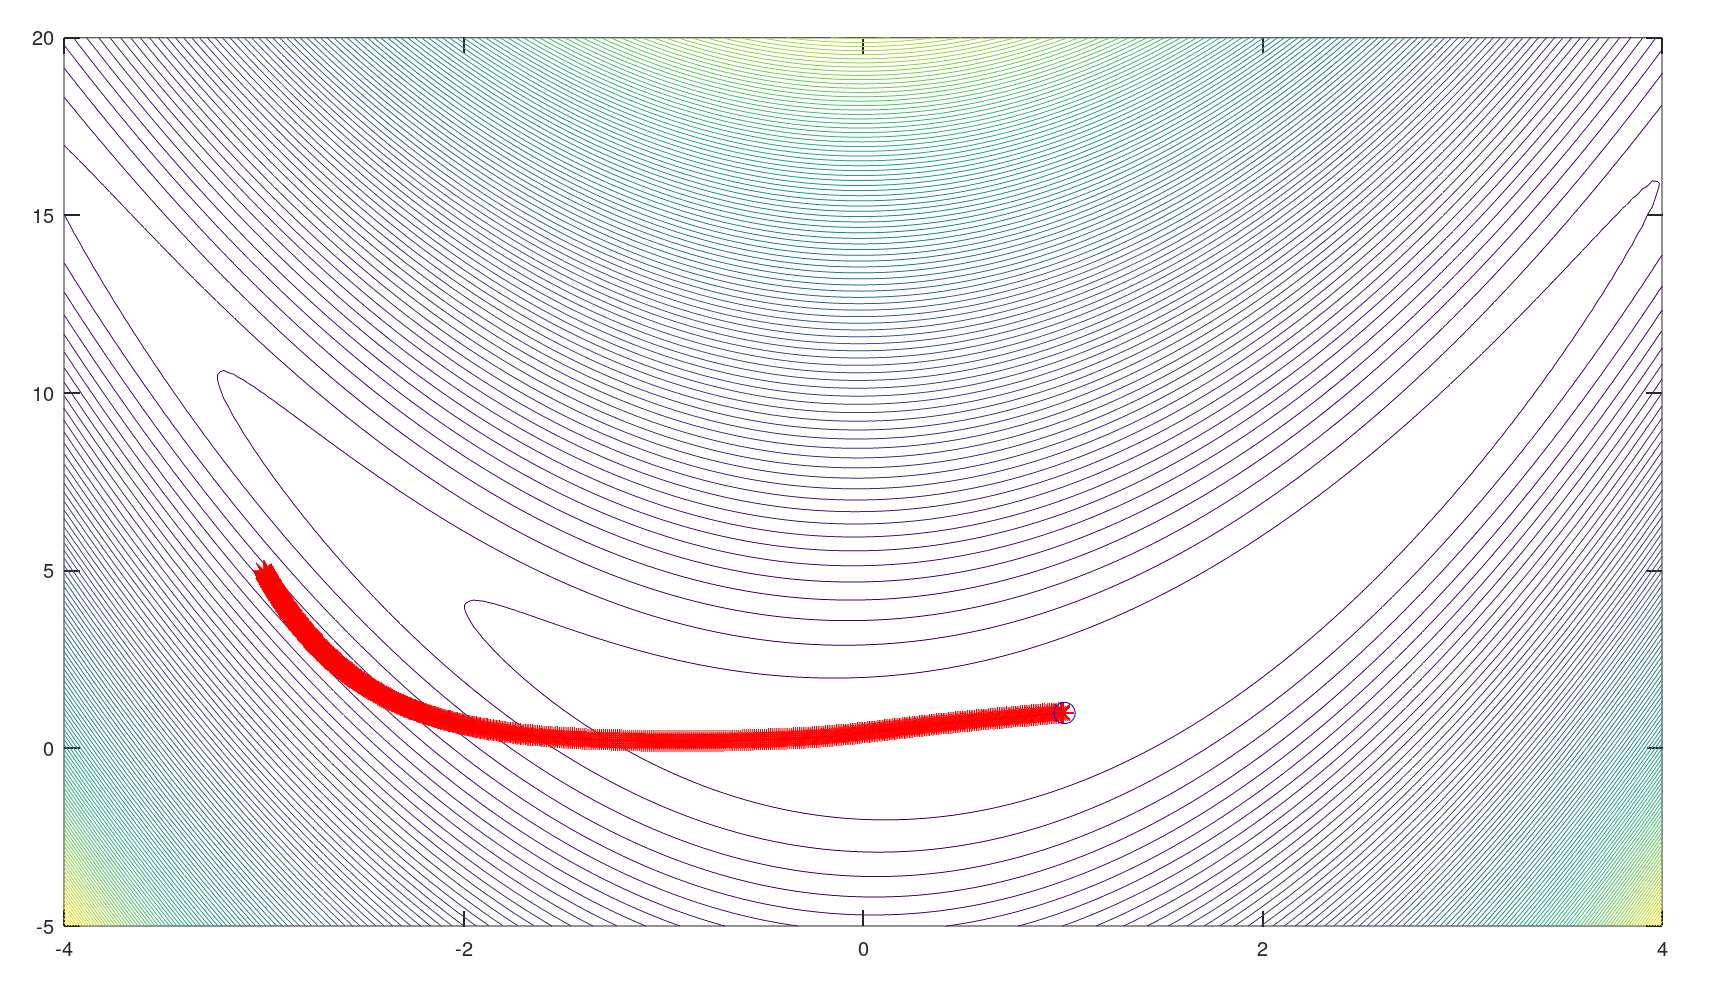
\includegraphics[width=7cm, height=4cm]{pasFixe10moins2}
			\caption{Descente de pas $10^{-2}$}
		\end{figure}
		
		\begin{figure}[H]
			\centering
			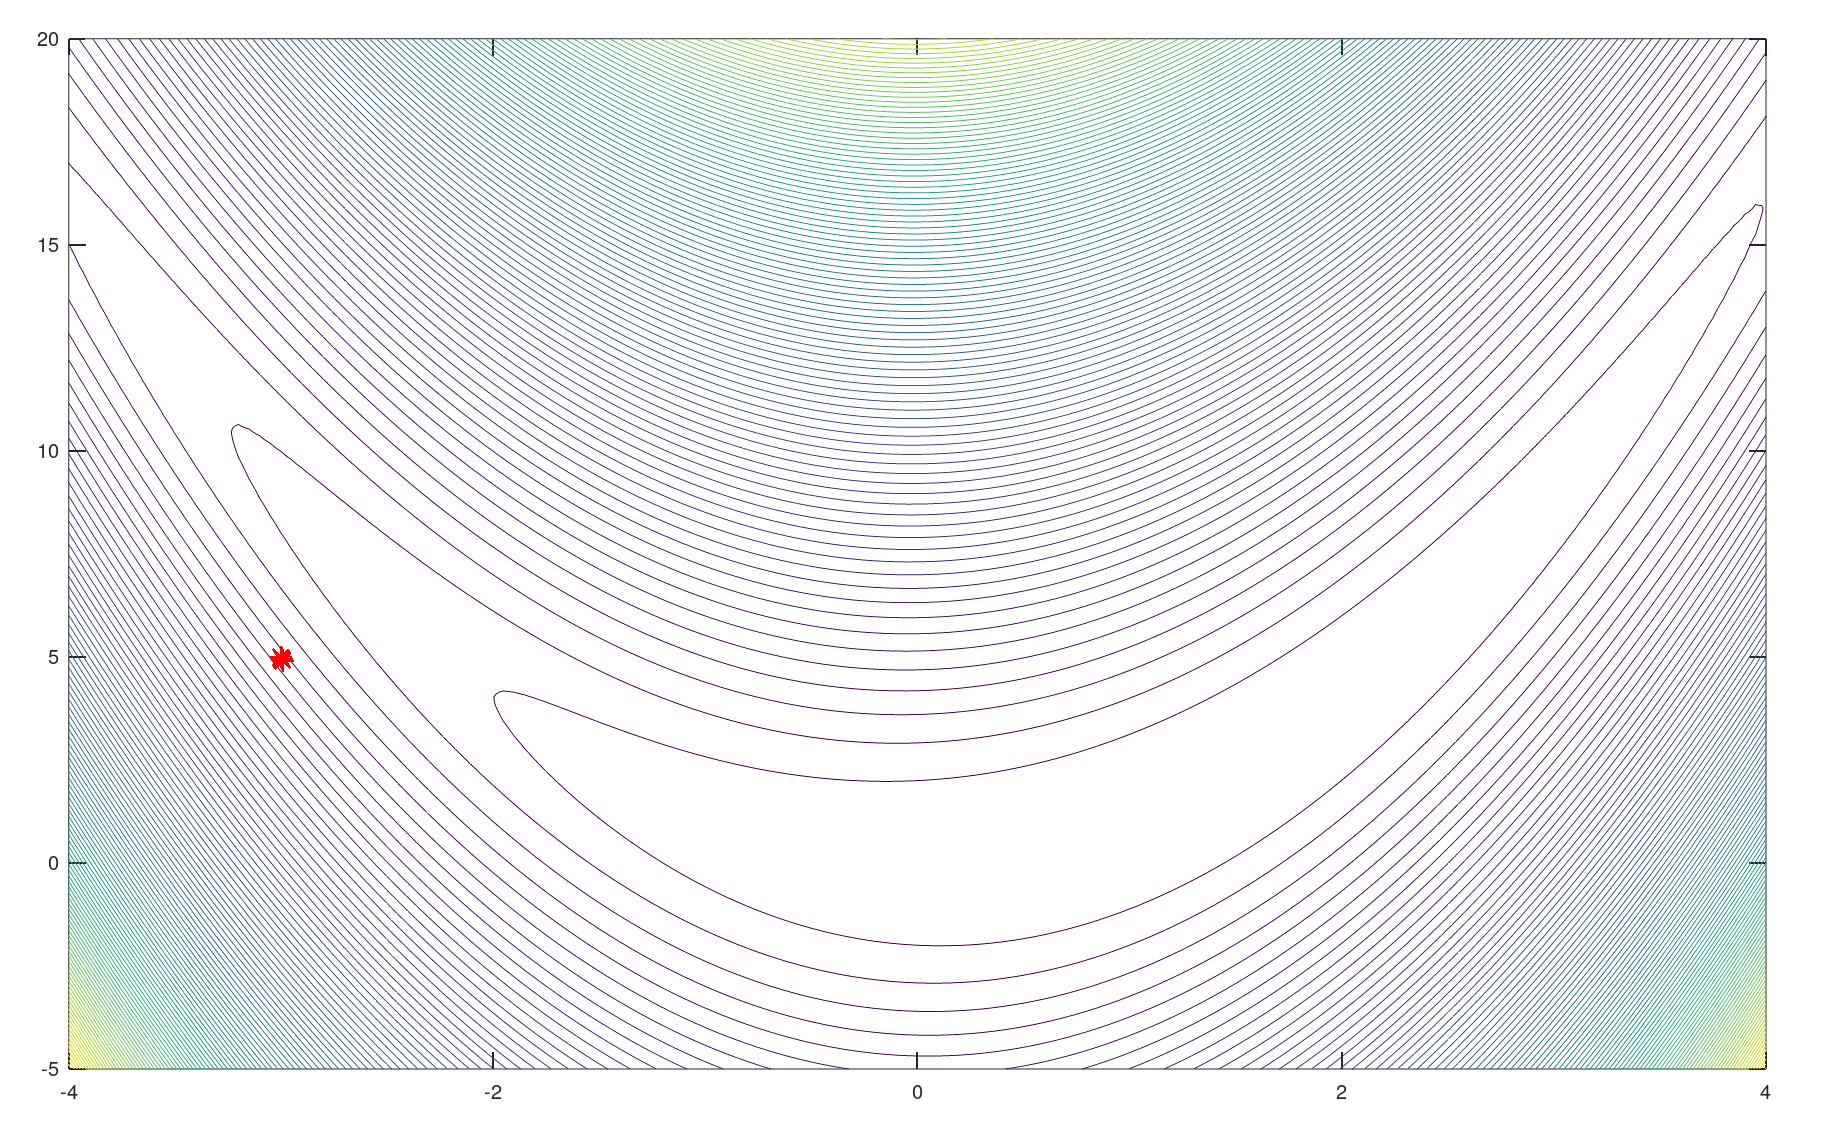
\includegraphics[width=7cm, height=4cm]{pasFixe10moins4}
			\caption{Descente de pas $10^{-4}$}
		\end{figure}
		
		On remarque qu'avec le pas de $10^{-4}$, les 1000 itérations ne sont pas suffisante pour tendre vers $ x_h$.
		\\On ajoute alors une recherche de pas par une technique de rebroussement avec un taux $\beta = 0.75$ pour assurer la condition d'Armijo avec $c=10^-4$
	
	\newpage
	\section{Ajustement d'une courbe non-linéaire}
		
	\newpage
	\section{Débruitage d’un signal par minimisation d ’un critère composite}
	
	\newpage
	\section{Inversion numérique d’une transformée de Laplace par optimisation sous contraintes}
\end{document}